\documentclass[a4paper,12pt]{article}
\usepackage[utf8]{inputenc}
\usepackage[T2A]{fontenc}
\usepackage[english, russian]{babel}
\usepackage{amsthm}
\usepackage{amsmath}
\usepackage{amssymb}
\usepackage{tikz}
\usepackage{textcomp}
\usepackage{esint}
\usepackage[unicode]{hyperref}
\usepackage{indentfirst}
\usepackage{algorithm}
\usepackage[noend]{algpseudocode}
\usepackage{amsmath,amsfonts,amssymb,amsthm,mathtools}
\usetikzlibrary{positioning,arrows}
\usepackage{graphicx}
\setlength{\topmargin}{-0.5in}
\setlength{\textheight}{9.1in}
\setlength{\oddsidemargin}{-0.4in}
\setlength{\evensidemargin}{-0.4in}
\setlength{\textwidth}{7in}
\setlength{\parindent}{0ex}
\setlength{\parskip}{1ex}
\usepackage{siunitx}
\usepackage{wrapfig}

\usepackage{multicol}
\usetikzlibrary{trees}
\usepackage{fancyhdr}
\usepackage{gensymb}

\newcommand{\bbR}{\mathbb R}
\newcommand{\eps}{\varepsilon}
\newcommand{\bbN}{\mathbb N}
\newcommand{\dif}{\mathrm{d}}

\pagestyle{fancy}
\makeatletter
\fancyhead[L]{}

\fancyfoot[R]{\thepage}
\fancyfoot[C]{}

\renewcommand{\maketitle}{
	\noindent{\bfseries\scshape\large\@title\ \mdseries\upshape}\par
	\noindent {\large\itshape\@author}
	\vskip 2ex}
\makeatother




\begin{document}
	
\Large \textbf { \begin{center}
		Работа 2.2\\ Изучение спектров атома водорода\\
		Селюгин Михаил, 876 \\
\end{center}}


	\section{Теория вопроса}
	Атом водорода является простейшей атомной системой и для него уравнение Шредингера может быть решено точно. Поэтому спектр атома водорода является предметом тщательного исследования.
	
	Длина волн спектральных линий водородоподобного атома описывается формулой Бальмера
	$$\frac1{\lambda_{mn} } = RZ^2\left(\frac1{n^2} - \frac1{m^2}\right),$$
	где $R$ --- постоянная Ридберга.
	
	Для объяснения спектра атома водорода Нильс Бор предложил следующие постулаты:
	\begin{itemize}
		\item из всех возможных орбит в атоме осуществляются только некоторые стационарные орбиты, при движении по которым электрон не излучает энергии;
		\item момент количества движения по стационарным орбитам кратен величине постоянной Планка, т.~е. 
		$$L = n\hbar$$ \newpage
		\item излучение или поглощение энергии происходит при переходе из одного стационарного состояния в другое, при этом частота излучаемого света удовлетворяет условию:
		$$h\nu = E_2-E_2$$
	\end{itemize}
\begin{wrapfigure}{l}{0.5\linewidth} %обтекание текстом
	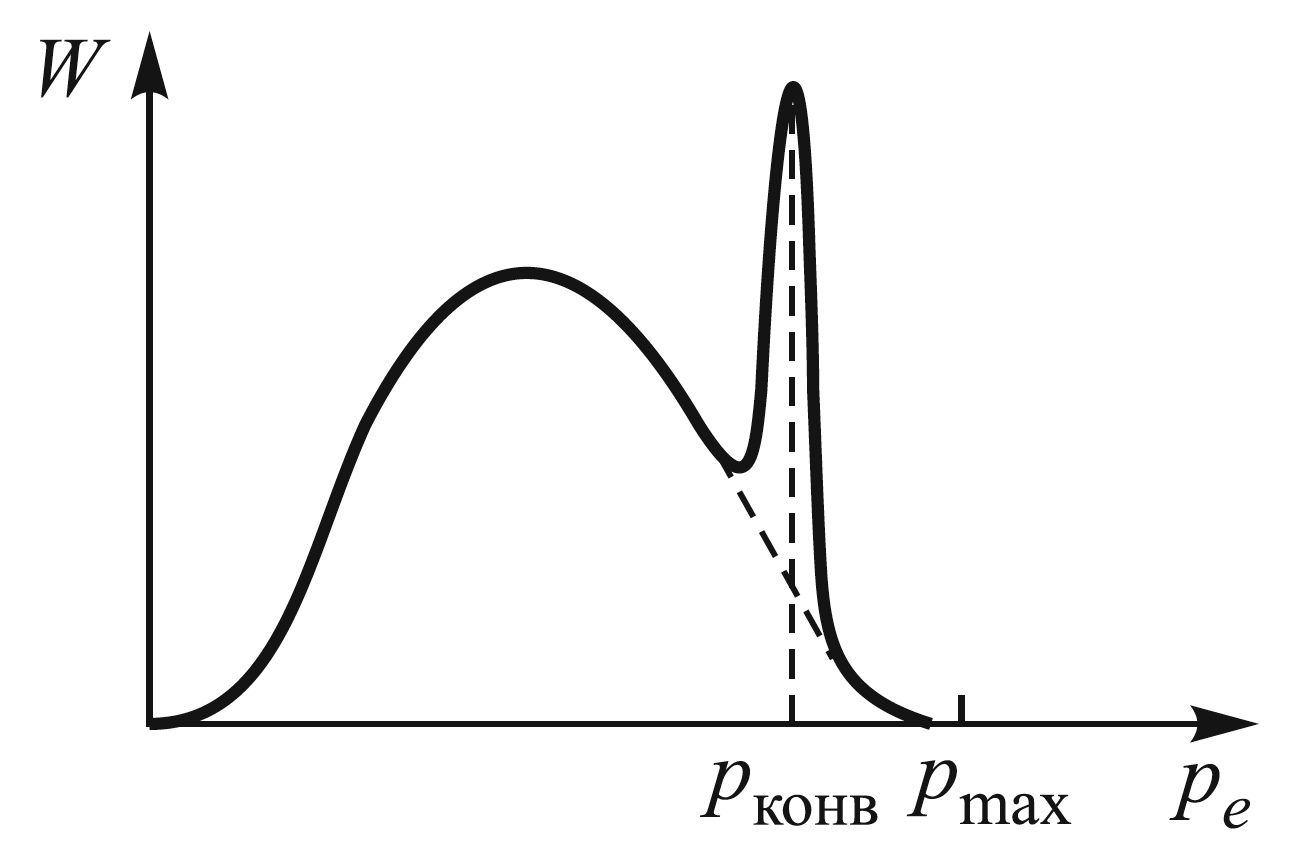
\includegraphics[width = 0.9\linewidth]{spektr.png}
\end{wrapfigure}
В таком случае энергетические состояния определяются выражением 
$$E_n = -\frac{m_e e^4Z^2}{2\hbar^2} \frac1{n^2}$$

Рассмотрев энергию как сумму потенциальной и кинетической составляющих, найдем энергию основного и возбужденных состояний, имеем
$$E = -\frac{ m_e e^4Z^2}{2\hbar^2} = -RZ^2$$
$$E_n = -R \frac{Z^2}{n^2}$$

Утверждение о том, что на орбите должно укладываться целое число  волн де Бройля соотвествует второму постулату Бора.

\newpage

\section{Экспериментальная установка}

Для измерения длин волн спектральных линий в работе используется стеклянно-призменный монохроматор-спектрометр УМ-2.
\begin{wrapfigure}{l}{0.65\linewidth} %обтекание текстом
	\includegraphics[width = \linewidth]{UM-2.png}
\end{wrapfigure}
\begin{enumerate}
	\item щель
	\item колл. объектив
	\item спектр. призма
	\item объектив
	\item окуляр
	\item столик
	\item [7-9.] винты
	\item[10.] указатель
	\item[11.] корпус
	\item[Л] --- источник
	\item[К] --- конденсор
\end{enumerate}
~\

~\

~\

~\

\newpage

\section{Ход работы}

{\bf 1. } Была произведена градуировка спектрометра УМ-2 по спектрам неона и ртути:

\includegraphics[width=0.6\linewidth]{NeHg.png}
\newpage
{\bf 2. } Был также снят спектр водорода 

\includegraphics[width=0.7\linewidth]{H.png}

{\bf 3. } На основании градуировки был построен график, на котором вертикальными линиями отмечены спектральные линии водорода. Точки пересечения линий с графиком позволяют определить длину волны.

\includegraphics[width=\linewidth]{graduir.png}
\newpage 
{\bf 4. }
Из градуировочного графика для каждой линии была определена длина волны. 
Принимая во внимание погрешность определения положения спектральной линии и погрешность градуировочного графика, была выбрана $\delta \lambda = 10A$.

\includegraphics[width=0.7\linewidth]{H_spektr.png}

{\bf 5. } Из формулы Бальмера
	$$\frac1{\lambda_{mn} } = RZ^2\left(\frac1{n^2} - \frac1{m^2}\right)$$
В данном случае $n=2,\ m = 3,4,5$.
Отсюда следуют соотношения между длинами волн, которые с высокой точностью подтверждаются экспериментом:
$$\left(\frac{\lambda_{42}}{\lambda_{32}}\right)_{th} \approx 0,741; \ \left(\frac{\lambda_{42}}{\lambda_{32}}\right)_{exp} \approx 0,745$$
$$\left(\frac{\lambda_{52}}{\lambda_{32}}\right)_{th} \approx 0,661; \ \left(\frac{\lambda_{52}}{\lambda_{32}}\right)_{exp} \approx 0,664$$
$$\left(\frac{\lambda_{52}}{\lambda_{42}}\right)_{th} \approx 0,893; \ \left(\frac{\lambda_{52}}{\lambda_{42}}\right)_{exp} \approx 0,891$$

{\bf 6. } Рассчитаем, наконец, постоянную Ридберга по каждой спектральной линии. Воспользуемся снова формулой Бальмера для водородопобных атомов.
$$ R = \frac1{\lambda_{mn}} : \left(\frac1{n^2} - \frac1{m^2}\right)$$

$$R_{\alpha} = (1,098 \pm 0,002)\cdot10^5 cm^{-1}$$
$$R_{\beta} = (1,0969 \pm 0,0013)\cdot10^5 cm^{-1}$$
$$R_{\gamma} = (1,0971 \pm 0,0012)\cdot10^5 cm^{-1}$$

Погрешность: $\eps_R = \eps_{\lambda}$ 

Тогда, усредняя, имеем $R = (1,097 \pm  0,002)\cdot10^5 cm^{-1}\ (\eps = 0,18\%)$

\section{Вывод}
В работе был исследован спектр водорода с помощью градуированных спектров ртути и неона. Были получены длины волн спектральных линий водорода, экспериментально подтверждена формула Бальмера и получено верное, в пределах погрешности, значение постоянной Ридберга.
$$R_{exp} = (1,097 \pm  0,002)\cdot10^5 cm^{-1}, \ R_{th} = 1,0968\cdot10^5 cm^{-1}$$
\end{document}